\documentclass[11pt]{article}

% Change "review" to "final" for the camera-ready version, or to "preprint" for a non-anonymous version.
\usepackage[review]{acl}

\usepackage{times}
\usepackage{latexsym}
\usepackage[T1]{fontenc}
\usepackage[utf8]{inputenc}
\usepackage{microtype}
\usepackage{graphicx}

\usepackage{amsmath,amssymb,amsthm,mathtools,bm}
\usepackage{booktabs,multirow,colortbl}
\usepackage{algorithm}
\usepackage[noend]{algpseudocode}
\usepackage{enumitem}
\usepackage{pifont}

\definecolor{oursrow}{HTML}{FDF0E9}
\newcommand{\method}{ForkOPD}
\newcommand{\tabinput}[1]{\csname @@input\endcsname #1 }
\newcommand{\Vt}{\tilde V}
\newcommand{\Ah}{\hat A}
\newcommand{\Yh}{\hat Y}
\newcommand{\piold}{\pi_{\mathrm{old}}}
\newcommand{\E}{\mathbb{E}}
\newcommand{\Var}{\mathrm{Var}}
\newcommand{\G}{\mathcal{G}}
\newcommand{\clip}{\operatorname{clip}}
\newcommand{\lamu}{\lambda^\star_{\mathrm u}}
\newcommand{\lamc}{\lambda^\star_{\mathrm c}}
\newcommand{\etac}{\eta_{\mathrm c}}

\newtheorem{lemma}{Lemma}
\newtheorem{theorem}{Theorem}
\newtheorem{proposition}{Proposition}
\theoremstyle{remark}
\newtheorem{remark}{Remark}

\setlist{leftmargin=*,itemsep=1pt,topsep=2pt,parsep=0pt}
\renewcommand{\topfraction}{0.9}
\renewcommand{\dbltopfraction}{0.9}
\renewcommand{\textfraction}{0.1}
\renewcommand{\floatpagefraction}{0.85}
\renewcommand{\dblfloatpagefraction}{0.85}
\setcounter{topnumber}{3}
\setcounter{dbltopnumber}{3}

\title{ForkOPD: Trust, but Rectify Privileged Teachers\\with Randomized Verified Forks}

\author{Anonymous ACL submission}

\begin{document}
\maketitle

\begin{abstract}
Reinforcement learning with verifiable rewards scores a whole reasoning trace with one bit, so per-step credit needs an estimate of how each step changed the chance of success. On-policy self-distillation reads that estimate off a privileged teacher: the same policy shown a reference solution. Measured against Monte Carlo values on Qwen3.5-9B, this hindsight signal is informative (Spearman 0.62), fades during training (0.38 after 400 steps), and errs most on near-miss prefixes that copy the reference and then fail. We therefore treat the teacher as a predictor and correct it. Following prediction-powered inference, \method{} (fork-rectified on-policy distillation) combines the teacher's prediction with a few verified continuations at randomly chosen segment boundaries. Its step values are conditionally unbiased for any predictor, as is the unclipped gradient estimate at the sampling policy; its trust coefficient and fork probabilities have closed forms; and it estimates online the share of predictor-dependent variance that hindsight removes. At a matched generation budget, \method{} improves the five-benchmark average by 3.0--4.3 points over DAPO on three base models and 2.0--2.8 over the strongest baseline (ten on Qwen3.5-9B, six on the others). With half of the references corrupted it loses 0.9 points, while methods that distill from or reweight with the uncorrected teacher lose 4.8--14.2.
\end{abstract}

\begin{figure*}[t]
  \centering
  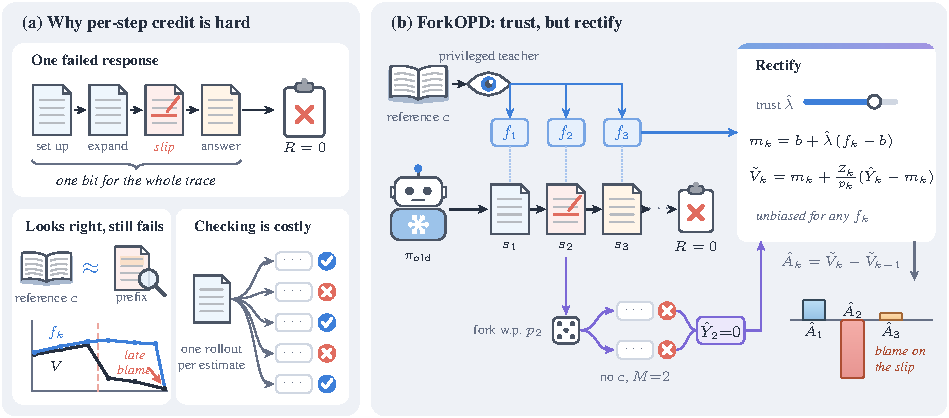
\includegraphics[width=\textwidth]{figures/fig1_overview.pdf}
  \caption{\textbf{Why per-step credit is hard, and how \method{} assigns it.} (a)~The verifier returns one bit for the whole response. A prefix that resembles the reference $c$ can already be lost, so the hindsight prediction $f_k$ stays high past the slip and the blame arrives late; checking every prefix with rollouts costs one rollout per estimate. (b)~\method{} predicts $f_k$ at every boundary with one pass of the privileged teacher, forks a few boundaries at random ($s_2$ here, with $M{=}2$ continuations sampled without $c$), and rectifies the predictions with the verified outcomes, so the blame lands on the slip.}
  \label{fig:overview}
\end{figure*}

% =====================================================================
\section{Introduction}
% =====================================================================

Reinforcement learning with verifiable rewards (RLVR) drives most recent progress in mathematical and programming reasoning \citep{guo2025deepseekr1,yu2025dapo}. A response can run for thousands of tokens, and the verifier returns one bit at the end. GRPO \citep{shao2024deepseekmath} and its variants spread that bit evenly over the response, so a careless sign error and the idea that solved the problem receive the same update. Finer credit needs the value of each intermediate state: the probability that the policy succeeds from that prefix.

Two families estimate this value. Resampling methods restart from a prefix and average verified continuations \citep{kazemnejad2025vineppo}, or spend the same budget at chosen branch points \citep{hou2025treerl,samanta2026resets}. Their estimates are unbiased, and each one costs a rollout. Reading methods perform on-policy self-distillation: they condition the policy on a reference solution to obtain a privileged teacher and use the teacher's per-token log-probability shift on the student's own samples as dense credit, at the price of one forward pass \citep{zhao2026opsd,hubotter2026sdpo}. Later variants let the verifier set the sign and use the teacher for magnitude \citep{yang2026rlsd,li2026hsd,huang2026flowbalance}.

Reading methods assume that the privileged score tracks the value it replaces. Against Monte Carlo values, a calibrated hindsight predictor reaches Spearman 0.62 on the initial policy and 0.38 after 400 steps of RL. Its largest errors sit on near misses (Figure~\ref{fig:overview}): prefixes that follow the reference and already contain a mistake the policy tends to repeat. Hindsight keeps predicting success there and blames the last segment for 63\% of failures (oracle: 18\%), and gating by the verifier fixes the sign of a response but not this misplacement.

We therefore use hindsight as a predictor of value and correct it where it errs, following prediction-powered inference \citep{angelopoulos2023ppi,zrnic2024active}, where a few gold labels placed with known probabilities remove the bias of many cheap predictions. In \method{}, short for fork-rectified on-policy distillation (Figure~\ref{fig:method}), the privileged teacher predicts the value at every segment boundary, and a random subset of boundaries, favoring uncertain predictions, receives a few verified continuations without the reference. Each rectified value is the prediction, anchored at the group baseline and scaled by a trust coefficient, plus an inverse-probability-weighted correction, and segment credit is the difference of consecutive values. These values are conditionally unbiased for any predictor, so a stale or misleading teacher adds variance but no bias, and the unclipped policy-gradient estimate is unbiased at the sampling policy. The trust coefficient in $[0,1]$ and the fork probabilities have closed forms, and \method{} estimates from its own fork labels the share of predictor-dependent variance that hindsight removes.

We train Qwen3.5-4B, Qwen3.5-9B \citep{qwen35} and Olmo-3-7B \citep{olmo2025olmo3} from base checkpoints at a matched generation budget, against ten baselines on the 9B model and six on the others. \method{} raises the five-benchmark average by 3.6, 4.3 and 3.0 points over DAPO and by 2.4, 2.8 and 2.0 over the strongest baseline, HSD. It reaches DAPO's final accuracy with 43\% of the tokens and keeps Pass@256 on AIME 2026 5.1 points above the base model, where DAPO falls 3.1 below it. Our contributions are:
\begin{itemize}
\item A measurement of privileged hindsight as a value signal: informative, fading with training, and wrong on near misses (Section~\ref{sec:diagnosis}).
\item \method{}, a credit estimator with conditionally unbiased step values for any predictor, closed-form trust and forks, and an online estimate of the variance hindsight removes (Sections~\ref{sec:predictor}--\ref{sec:guarantees}).
\item Matched-budget experiments against ten baselines on Qwen3.5-9B and six on two other models, including gradient quality against oracle advantages and wrong references (Section~\ref{sec:experiments}).
\end{itemize}


% =====================================================================
\section{Related Work}
% =====================================================================

\paragraph{Credit assignment in RLVR.}
Group-relative methods \citep{shao2024deepseekmath,ahmadian2024back,yu2025dapo} assign one outcome to every token, and shrinkage across prompts lowers the variance of their baselines \citep{zeng2026shrinking}. VinePPO \citep{kazemnejad2025vineppo} replaced learned value networks, which rank reasoning steps poorly, with Monte Carlo continuations. Tree methods branch at high-entropy tokens \citep{hou2025treerl}, at steps with large attention mass \citep{liu2026attention}, at semantically divergent points \citep{zhao2026semantically}, or where expected gradient information is largest \citep{khomich2026epig}, and reset methods resample from a self-localized error \citep{samanta2026resets}. \method{} places its continuations at random with known probabilities and needs fewer of them because a predictor carries part of the estimate. Process reward models \citep{lightman2024verify,wang2024mathshepherd,setlur2025rewarding,yuan2025free} could serve as that predictor.

\paragraph{Privileged self-distillation.}
On-policy distillation \citep{agarwal2024onpolicy} became self-distillation once the teacher was the student conditioned on privileged context \citep{zhao2026opsd,hubotter2026sdpo}, which can suppress exploratory reasoning \citep{kim2026whyselfdistill}. Later methods let the verifier set the direction \citep{yang2026rlsd}, condition the teacher on successful peers \citep{li2026hsd}, contrast correct and incorrect teachers \citep{heakl2026cepo}, or fold the gated signal into a trajectory-balance target \citep{huang2026flowbalance}. OC-GRPO puts the privileged context into the rollout and corrects with importance weights \citep{agrawal2026ocgrpo}. \method{} keeps the reference out of every rollout and out of the update, and uses it only to predict values.

\paragraph{Prediction-powered and active inference.}
Prediction-powered inference \citep{angelopoulos2023ppi} gives valid estimates from many predictions and few labels. PPI++ \citep{angelopoulos2023ppipp} adds the power-tuning coefficient that becomes our $\lambda$, and active inference \citep{zrnic2024active} chooses which points to label using inverse-probability weights \citep{horvitz1952generalization} and Neyman-style allocation \citep{neyman1934two}. Unlike baselines as control variates \citep{greensmith2004variance}, \method{} estimates intermediate values with no observed outcome and creates their labels with forks; unlike asymmetric critics \citep{vapnik2009lupi,pinto2018asymmetric}, its privileged critic is the policy itself.

% =====================================================================
\section{Methodology}
\label{sec:method}
% =====================================================================

\begin{figure*}[t]
  \centering
  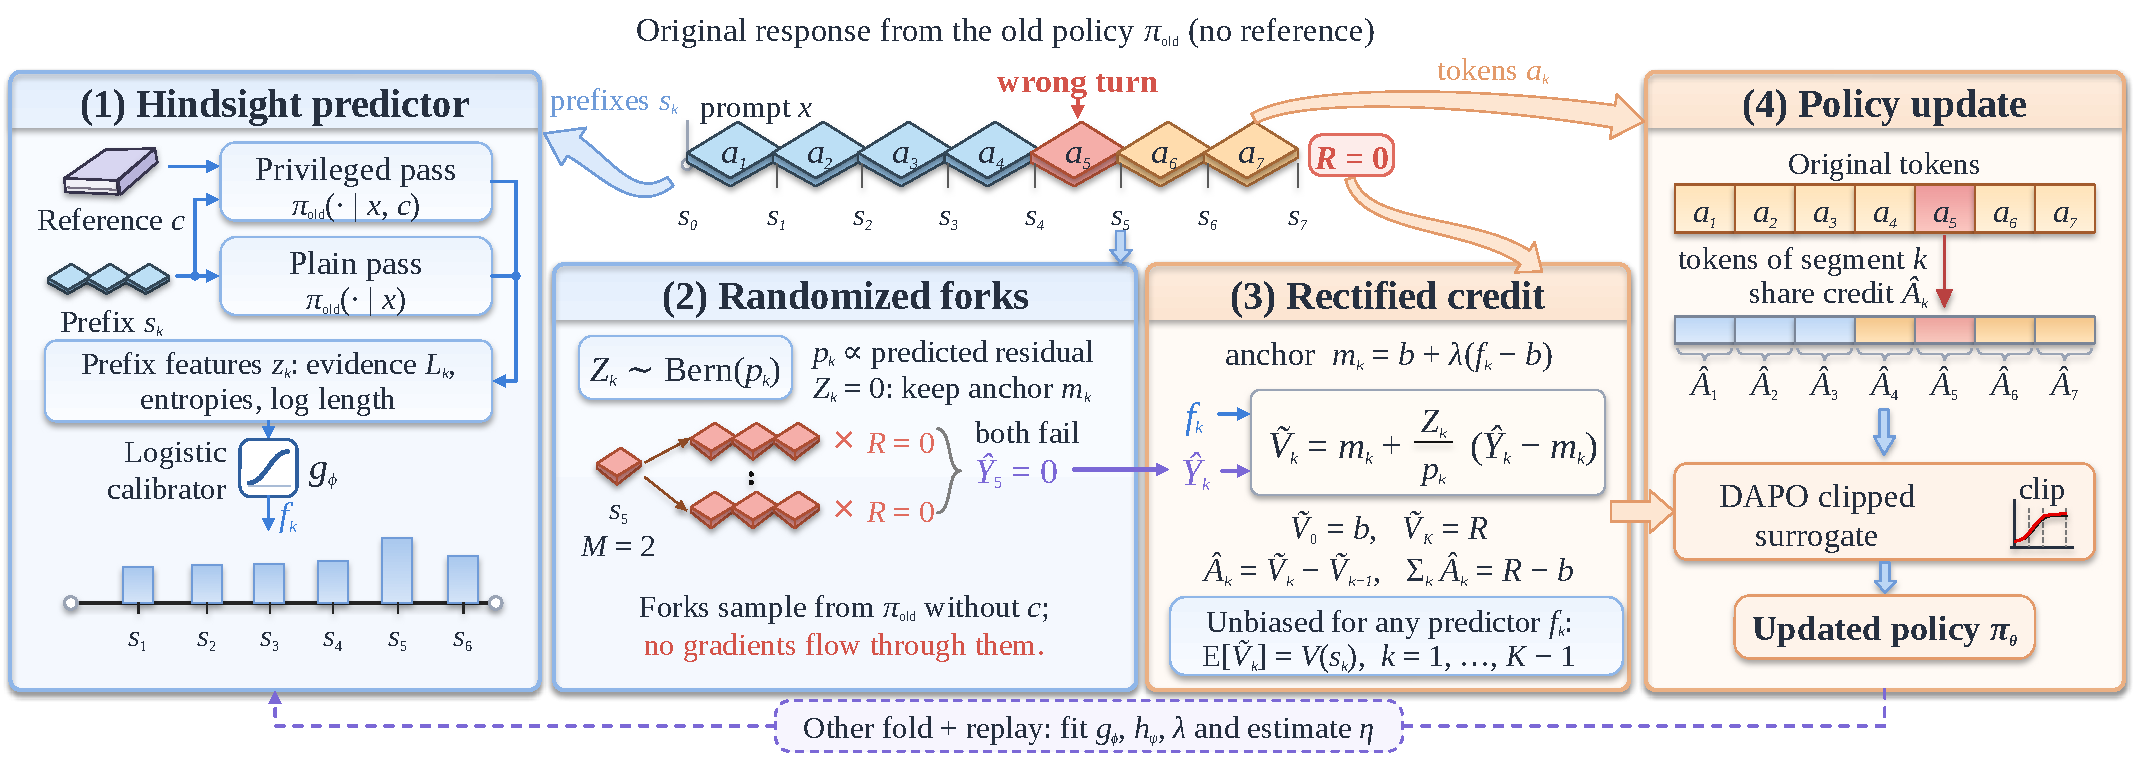
\includegraphics[width=\textwidth]{figures/fig2_method.pdf}
  \caption{\textbf{One iteration of \method{}.} \ding{172}~A privileged and a plain pass over each prefix give features $z_k$, and a logistic calibrator $g_\phi$ maps them to the prediction $f_k$. \ding{173}~Each boundary is forked independently with probability $p_k$. At $s_5$, both continuations sampled from $\piold$ without $c$ fail, so $\hat Y_5{=}0$. \ding{174}~The rectified values $\tilde V_k$ correct the anchor $m_k$ where a fork was taken, and their differences give the segment credit $\hat A_k$. \ding{175}~Every token of segment $k$ receives $\hat A_k$ in the DAPO update. Bottom: each prompt fold fits $g_\phi$, $h_\psi$ and $\hat\lambda$, and estimates $\hat\eta$, for the other fold.}
  \label{fig:method}
\end{figure*}

\subsection{Preliminaries}
\label{sec:prelim}

A policy $\pi_\theta$ answers a prompt $x$ with a response $y$, and a verifier returns $R(x,y)\in\{0,1\}$. We split $y$ into segments $a_1,\dots,a_K$ and write $s_k=(x,a_1,\dots,a_k)$, with $s_0=x$. A boundary is placed at the first double newline at least 64 tokens after the previous boundary, or after 1{,}024 tokens without one. Each decision depends only on the prefix, so boundaries are stopping times. With $\piold$ the policy that generated the batch, the value of a state is its probability of eventual success,
\begin{equation}
V(s_k) = \E_{y'\sim\piold(\cdot\mid s_k)}\bigl[R(x, s_k\oplus y')\bigr],
\label{eq:value}
\end{equation}
and $V(s_K)=R(x,y)$. Transitions are deterministic, so segment $a_k$ has advantage $A_k=V(s_k)-V(s_{k-1})$ and $\nabla_\theta J=\E\bigl[\sum_k A_k\nabla_\theta\log\pi_\theta(a_k\mid s_{k-1})\bigr]$. Each prompt is answered $N$ times, and $b$ is the leave-one-out mean reward of the other $N-1$ responses \citep{ahmadian2024back}.

A training prompt often comes with a reference solution $c$ that the deployed model never sees. Scoring the sampled tokens with $\piold$ conditioned on $c$ gives the hindsight evidence
\begin{equation}
L_k = \log\piold(a_{1:k}\mid x,c) - \log\piold(a_{1:k}\mid x),
\label{eq:evidence}
\end{equation}
the summed per-token log ratio $\ell_t$ up to boundary $k$. A prefix that agrees with $c$ has high $L_k$, and reading methods turn $\ell_t$ into credit.

\subsection{Motivation: how far can hindsight be trusted?}
\label{sec:diagnosis}

We freeze Qwen3.5-9B checkpoints from a DAPO run at steps 0, 200 and 400, sample 2{,}000 responses to held-out DeepMath prompts from each, and estimate every boundary's value with 64 verified continuations. The hindsight predictor is a logistic model on the features of Section~\ref{sec:predictor}, fit to oracle values on separate responses; a control omits $c$.

\begin{figure}[t]
  \centering
  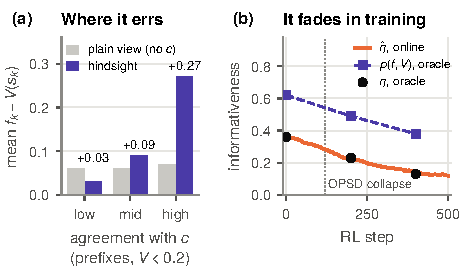
\includegraphics[width=\columnwidth]{figures/fig_diagnosis.pdf}
  \caption{\textbf{Hindsight against oracle values} (Qwen3.5-9B; 64 continuations per boundary). \textbf{(a)}~Error of two calibrated predictors on low-value prefixes by agreement with the reference. \textbf{(b)}~Spearman correlation and $\eta$ (Theorem~\ref{thm:eta}) across a DAPO run, with \method{}'s online estimate $\hat\eta$ of $\etac\le\eta$.}
  \label{fig:diagnosis}
\end{figure}

\paragraph{The signal is informative and fades.}
At step 0 the hindsight predictor reaches Spearman $\rho=0.62$ with oracle values and the control 0.29. The correlation falls to 0.49 at step 200 and 0.38 at step 400, and the removable variance share $\eta$ (Theorem~\ref{thm:eta}) falls from 0.36 to 0.13 (Figure~\ref{fig:diagnosis}b). As RL sharpens the policy, $\ell_t$ shrinks on good and bad prefixes alike.

\paragraph{The error sits on near misses.}
On prefixes with $V(s_k)<0.2$, the control overestimates by 0.06 to 0.07 at every level of agreement with the reference, the usual regression to the mean (Figure~\ref{fig:diagnosis}a). Hindsight overestimates by 0.03 on prefixes that disagree with the reference and by 0.27 on the top tercile of agreement: prefixes that copied the reference and already contain a mistake the policy tends to repeat.

\paragraph{Blame lands late, and gating keeps it there.}
Credit $f_k-f_{k-1}$, with endpoints $b$ and $R$, puts the most negative segment of a failed response at its final segment in 63\% of failures, against 18\% under oracle advantages. Verifier gating gives a failed response negative total credit but still distributes it by hindsight: the rate is 41\% for RLSD-style gating and 33\% for HSD's peer-conditioned teacher.

\subsection{A hindsight value predictor}
\label{sec:predictor}

For each boundary we compute $z_k$ from one privileged forward pass and from the old-policy pass that DAPO already runs: the per-token evidence $L_k/t_k$, with $t_k$ the response tokens in $s_k$; its increment $L_k-L_{k-1}$; the mean plain-view entropy over $a_k$; the privileged-minus-plain entropy gap over $a_k$; and $\log t_k$. A six-parameter logistic model maps $z_k$ to $f_k=g_\phi(z_k)\in(0,1)$. It is fit on fork labels only, with cross-fitting: the prompts of a batch are split into two folds, and each fold is predicted by a calibrator fit on the other fold plus a replay buffer of the previous 20 batches. This keeps $f_k$ independent of the labels it is compared with, as Lemma~\ref{lem:unbiased} requires.

\subsection{Randomized forks}
\label{sec:forks}

At each interior boundary $k$ we draw $Z_k\sim\mathrm{Bernoulli}(p_k)$ independently. If $Z_k=1$, we sample $M$ continuations from $s_k$ with $\piold$ and without $c$, verify them, and record their mean $\Yh_k$. As in VinePPO, the continuations receive no gradient. Proposition~\ref{prop:variance} shows that the best $p_k$ grows with the expected squared error of the anchored prediction $m_k$ defined below, so a linear model $h_\psi$, cross-fitted like $g_\phi$, predicts that error beyond binomial noise from $z_k$. With a per-response budget $B$ and a floor $p_{\min}$,
\begin{equation}
\begin{gathered}
p_k = \min\bigl\{1,\ \max\bigl\{p_{\min},\ B\,u_k/{\textstyle\sum_j} u_j\bigr\}\bigr\},\\
u_k = \sqrt{f_k(1-f_k)/M + h_\psi(z_k)} .
\end{gathered}
\label{eq:pk}
\end{equation}
The floor bounds every importance weight by $1/p_{\min}$. Equation~\eqref{eq:pk} clips without renormalizing, so $B$ is nominal and the $p_k$ need not sum to it (Appendix~\ref{app:proofs}); budgets count realized forks. We use $B=1$, $M=2$ and $p_{\min}=0.025$, which gives 1.06 forks per response.

\subsection{Rectified values and segment credit}
\label{sec:rectify}

The prediction enters through an anchor $m_k=b+\lambda(f_k-b)$ that shrinks it toward the group baseline by a trust coefficient $\lambda\in[0,1]$. The rectified value at an interior boundary is
\begin{equation}
\Vt_k = m_k + \frac{Z_k}{p_k}\bigl(\Yh_k - m_k\bigr),
\label{eq:rectified}
\end{equation}
with $\Vt_0=b$ and $\Vt_K=R(x,y)$. An unforked boundary keeps the anchor. At a forked one the anchor cancels in expectation and the verified mean takes over. Segment credit is
\begin{equation}
\Ah_k = \Vt_k - \Vt_{k-1},\qquad \sum_{k=1}^{K}\Ah_k = R(x,y) - b ,
\label{eq:credit}
\end{equation}
and every token of segment $k$ receives advantage $\Ah_k$ in DAPO's clipped surrogate. Segment credits sum to the RLOO advantage, and hindsight and forks decide how it is split among segments; summed over tokens, each $\Ah_k$ is weighted by the length $|a_k|$ (Appendix~\ref{app:impl}).

\paragraph{Trust coefficient.}
With $\omega_k=(1-p_k)/p_k$, the summed variance of Equation~\eqref{eq:rectified} over a batch is minimized over $\lambda\in\mathbb{R}$ by a weighted regression slope $\lamu$ of $V_k-b$ on $f_k-b$, and over $[0,1]$ by $\lamc=\clip(\lamu,0,1)$ (Proposition~\ref{prop:variance}). We estimate the slope on the other fold,
\begin{equation}
\hat\lambda = \frac{\sum \omega_k\,(f_k-b)\,\frac{Z_k}{p_k}(\Yh_k - b)}{\sum \omega_k\,(f_k-b)^2},
\label{eq:lambda}
\end{equation}
and clip it to $[0,1]$. Centering at $b$ makes $\lambda$ a slope: a calibrated predictor that only knows the base rate gets $\lambda\approx0$, whereas the uncentered form $m_k=\lambda f_k$ would give it $\lambda\approx1$. We also log $\hat\eta$, an estimate of the variance share $\etac$ removed by the clipped coefficient (Theorem~\ref{thm:eta}; Appendix~\ref{app:proofs}).

\paragraph{Cost.}
Scoring adds one forward pass with $c$ in context. Forks start partway through a response, so with $N=8$ a prompt costs 15.6 response-equivalents of generation, close to DAPO's 16 (Algorithm~\ref{alg:precise}, Appendix~\ref{app:impl}).

\subsection{Guarantees}
\label{sec:guarantees}

Let $\G$ contain the response, $c$, the other responses of the group, and all labels from the other fold and from earlier batches. By construction, $f_k$, $p_k$, $\hat\lambda$ and $b$ are $\G$-measurable. Proofs are in Appendix~\ref{app:proofs}.

\begin{lemma}[Unbiased rectified value]\label{lem:unbiased}
If $p_k>0$ and the continuations at $s_k$ are drawn from $\piold(\cdot\mid s_k)$ independently of $\G$ and $Z_k$, then $\E[\Vt_k\mid\G]=V(s_k)$ for every $\G$-measurable $f_k$, $\lambda$ and $b$.
\end{lemma}

\begin{theorem}[Unbiased policy gradient]\label{thm:grad}
Under the conditions of Lemma~\ref{lem:unbiased}, if boundaries are stopping times, then $\hat g=\sum_k\Ah_k\nabla_\theta\log\pi_\theta(a_k\mid s_{k-1})$ satisfies $\E[\hat g]=\nabla_\theta J(\theta_{\mathrm{old}})$ at $\theta=\theta_{\mathrm{old}}$.
\end{theorem}

The lemma places no condition on $f_k$: a miscalibrated, stale or adversarial predictor changes the variance of $\Vt_k$ and leaves its conditional mean alone. The theorem needs causal boundaries, because a rule that merges segments after seeing the response makes boundaries depend on later tokens, which correlate with the outcome.

\begin{proposition}[Variance and optimal design]\label{prop:variance}
With $V_k=V(s_k)$ and $\sigma_k^2=V_k(1-V_k)/M$,
\begin{equation}
\Var(\Vt_k\mid\G)=\frac{\sigma_k^2}{p_k}+\omega_k\,(V_k-m_k)^2 .
\label{eq:variance}
\end{equation}
Let $A$, $C$ and $D$ be the $\omega$-weighted sums over $k$ of $(f_k-b)^2$, $(f_k-b)(V_k-b)$ and $(V_k-b)^2$. For fixed $\{p_k\}$, the summed variance is a term free of $\lambda$ plus the predictor-dependent component $S(\lambda)=D-2\lambda C+\lambda^2A$. If $A>0$, $S$ is minimized over $\mathbb{R}$ by $\lamu=C/A$ and over $[0,1]$ by $\lamc=\clip(C/A,0,1)$; if $A=0$, $S\equiv D$ and we take $\lamc=0$. The numerator of Equation~\eqref{eq:lambda} is unbiased for $C$. For fixed anchors and an exact budget $B$, the summed variance is minimized by $p_k^\star\propto\sqrt{\sigma_k^2+(V_k-m_k)^2}$, truncated at one.
\end{proposition}

\begin{theorem}[Variance saved by hindsight]\label{thm:eta}
For $A,D>0$, $S(\lamu)=(1-\eta)\,S(0)$ and $S(\lamc)=(1-\etac)\,S(0)$ with $\eta=C^2/(AD)$ and $\etac=(2\lamc C-(\lamc)^2A)/D$. Also, $0\le\etac\le\eta\le1$, with $\etac=\eta$ exactly when $\lamu\in[0,1]$. For $A=0$ or $D=0$, nothing can be removed and we set $\eta=\etac=0$.
\end{theorem}

At $\lambda=0$, \method{} reduces to inverse-probability weighting with the same forks around the group baseline, so at $\lamc$ its variance never exceeds that of forks alone. $\eta$ is a squared weighted correlation around the baseline and measures information rather than calibration; an anticorrelated predictor has $\eta>0$ but $\etac=0$ (Appendix~\ref{app:proofs}). When $\lamu\in[0,1]$, the cross-fitted $\hat\lambda$ gives $S(\hat\lambda)-S(\lamc)$ of order $1/n$ in the number of fork labels per fold \citep{angelopoulos2023ppipp}.

% =====================================================================
\section{Experiments}
\label{sec:experiments}
% =====================================================================

\subsection{Experimental Setup}

\subsubsection{Benchmarks and Baselines}

\paragraph{Models and data.}
We train from base checkpoints so that every gain comes from RL: Qwen3.5-4B-Base and Qwen3.5-9B-Base \citep{qwen35}, hybrids of Gated DeltaNet and attention layers, and Olmo-3-7B \citep{olmo2025olmo3}, whose open pretraining data can be checked for contamination. For mathematics we filter DeepMath-103K \citep{he2026deepmath} to problems of difficulty six or above whose base-model pass rate over eight samples is strictly between 0 and 1, which leaves 24.3K prompts with three R1 solutions each, one of which we use as $c$. For programming we use the 12.1K human-seeded problems of rStar-Coder \citep{liu2025rstarcoder}, with oracle solutions as $c$ and verified tests.

\paragraph{Evaluation.}
Mathematics: AIME 2026 and HMMT February 2026 (released after or within weeks of the base models), BeyondAIME, IMO-AnswerBench \citep{luong2025robust} and AIME 2025. Programming: LiveCodeBench v6 \citep{jain2025livecodebench} and LCB-2026, 187 AtCoder and Codeforces problems from January to August 2026 collected with the LiveCodeBench pipeline. Out of domain: GPQA-Diamond \citep{rein2024gpqa}. We report avg@16 on AIME and HMMT and avg@8 elsewhere, sampling at temperature 1.0 and top-$p$ 0.95 with an 8{,}192-token budget.

\paragraph{Baselines and budget.}
We group ten baselines, all run on Qwen3.5-9B and six on the other models (Table~\ref{tab:other}), by how they obtain credit: outcome only (GRPO, DAPO; \citealp{shao2024deepseekmath,yu2025dapo}), resampling (VinePPO, TreeRL, SRPO), privileged self-distillation (OPSD, RLSD, HSD), privileged rollouts with importance correction (OC-GRPO) and distributional (FlowBalance), with citations in Section~2. All run in verl \citep{sheng2025hybridflow} on a shared DAPO backbone with the same data, verifier, length cap and optimizer, with their own coefficients tuned on a held-out split (Appendix~\ref{app:baselines}). We match generation per step, counting every continuation: methods without forks use $N=16$, \method{} uses $N=8$ with $B=1$ and $M=2$, and VinePPO, TreeRL and SRPO use $N=8$ plus their own continuations. A 9B run generates about $3.9\times10^9$ tokens in 500 steps (Appendix~\ref{app:budget}).

\subsubsection{Implementation Details}

We train Qwen3.5-9B for 500 steps (fewer for the other models) with 128 prompts per step, learning rate $10^{-6}$, DAPO clipping $(0.2,0.28)$, no KL penalty and responses up to 8{,}192 tokens, on 64 H100 GPUs. Qwen3.5-9B responses have 13.2 segments on average. Results are means over three seeds (Appendix~\ref{app:stats}); Appendix~\ref{app:impl} lists all settings.

\begin{table*}[t]
\centering
\small
\setlength{\tabcolsep}{6pt}
\begin{tabular}{llcccccc c}
\toprule
Family & Method & AIME26 & HMMT26 & BeyondAIME & IMO-AB & AIME25 & Avg. & $\Delta$ \\
\midrule
\tabinput{tables/main_9b.tex}
\bottomrule
\end{tabular}
\caption{\textbf{Mathematical reasoning on Qwen3.5-9B} trained from the base checkpoint with about $3.9\times10^9$ generated tokens per method. avg@16 for AIME and HMMT, avg@8 otherwise; mean of three seeds. Best in \textbf{bold}, second \underline{underlined}; $\Delta$ is the change in average relative to DAPO.}
\label{tab:main}
\end{table*}

\subsection{Main Results}

\method{} is best on all five benchmarks (Table~\ref{tab:main}) and raises the 9B average by 4.28 points over DAPO, 2.76 over HSD and 3.16 over SRPO. A paired permutation test against HSD on the 590 pooled problems gives $p=0.003$.

The baselines sort by how much they trust the privileged view. OPSD distills toward it and ends 6.30 points below DAPO, its mean response length falling from 3.9K to 1.6K tokens \citep{kim2026whyselfdistill}. RLSD matches DAPO and FlowBalance gains 0.74. SRPO and HSD, which obtain intermediate outcomes through resets and successful peers, are the strongest baselines. VinePPO trails DAPO by 0.72 points: at a matched budget, forking at every boundary leaves it 36 prompts per step.

\begin{table}[t]
\centering
\small
\setlength{\tabcolsep}{2.6pt}
\begin{tabular}{lccccc}
\toprule
& \multicolumn{2}{c}{Math avg.} & \multicolumn{3}{c}{Qwen3.5-9B} \\
\cmidrule(lr){2-3}\cmidrule(lr){4-6}
Method & Qw-4B & Olmo & LCB v6 & LCB-26 & GPQA \\
\midrule
\tabinput{tables/other_models.tex}
\bottomrule
\end{tabular}
\caption{\textbf{Other base models and domains} (six baselines). Left: five-benchmark math average. Right: Qwen3.5-9B on programming (avg@8 pass rate) and on GPQA-Diamond with the math-trained checkpoints.}
\label{tab:other}
\end{table}

On Qwen3.5-4B and Olmo-3-7B (six baselines, Table~\ref{tab:other}), \method{} again leads, by 2.40 and 2.02 points over HSD. Olmo starts lower, so fewer of its prompts produce mixed outcomes and there is less credit to redistribute. On programming, where $c$ is an oracle program and the verifier runs unit tests, \method{} improves LiveCodeBench v6 by 2.5 points and the post-release LCB-2026 split by 2.2 over HSD. On GPQA-Diamond, which no method trains on, the math-trained checkpoints lie within 2.6 points of each other and \method{} is highest at 44.1.

\paragraph{Efficiency.}
\method{} reaches DAPO's final 9B average after 43\% of the token budget, against 74\% for HSD and 81\% for SRPO (Figure~\ref{fig:training}a), and after 55\% of DAPO's wall-clock time (Figure~\ref{fig:training}b). A full run takes 1.27 times as long as DAPO, because mid-response forks batch poorly and the privileged pass adds compute.

\begin{figure*}[t]
  \centering
  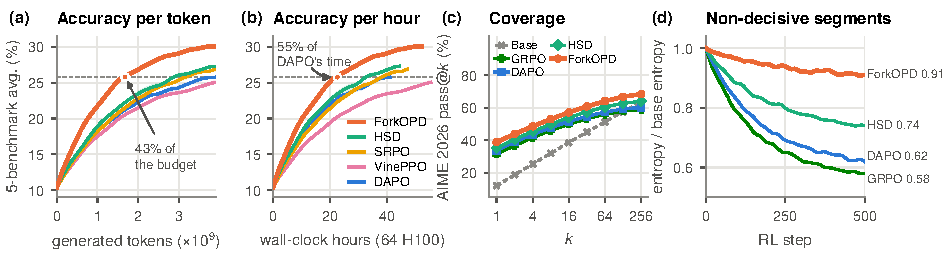
\includegraphics[width=\textwidth]{figures/fig3_training.pdf}
  \caption{\textbf{Training dynamics on Qwen3.5-9B.} \textbf{(a, b)}~Five-benchmark average against generated tokens and wall-clock hours on 64 H100 GPUs; bands span three seeds, the dashed line marks DAPO's final average. \textbf{(c)}~Pass@$k$ on AIME 2026 after training. \textbf{(d)}~Token entropy on non-decisive segments ($|A_k|<0.02$ under oracle values), relative to the base model.}
  \label{fig:training}
\end{figure*}

\subsection{Ablations}

\begin{table*}[t]
\centering
\small
\setlength{\tabcolsep}{4pt}
\begin{tabular}{llcr}
\toprule
Component & Variant & Avg. & \\
\midrule
\tabinput{tables/ablation_left.tex}
\bottomrule
\end{tabular}
\hfill
\begin{tabular}{llcr}
\toprule
Component & Variant & Avg. & \\
\midrule
\tabinput{tables/ablation_right.tex}
\bottomrule
\end{tabular}
\caption{\textbf{Ablations on Qwen3.5-4B} (five-benchmark average; full method 22.24, DAPO 18.60). Each row changes one component; gray: change from the full method. $^\dagger$One of three seeds diverged after step 300; mean of the other two. $^\ddagger$$h_\psi$ fit to total squared residuals, no $\hat\eta$ (App.~\ref{app:impl}).}
\label{tab:ablation}
\end{table*}

\paragraph{Rectification.}
Hindsight alone ($\lambda=1$, no forks) is 0.30 points above DAPO, forks alone ($\lambda=0$) 1.30, and the combination 3.64. Beyond the variance saving, clipping explains part of the gap: with forks alone the importance-weighted corrections carry the whole learning signal, and 27\% of their magnitude falls on tokens whose probability ratio is already clipped, against 9\% with the anchor. Centering matters too: the uncentered anchor $m_k=\lambda f_k$ loses 0.74. Fixed $\lambda=1$ loses 0.44 and $\lambda=0.5$ loses 0.94; the calibrator is fit on slightly stale labels, and $\hat\lambda$ follows its drifting slope.

\paragraph{Fork placement.}
Placing forks by predicted residual beats uniform placement by 1.14 points and entropy-based branching by 0.84. With $p_{\min}=0.025$ the median importance weight on forked boundaries is 6.8 and the 99th percentile 38. Without the floor, weights reached $1.4\times10^3$ and one seed diverged.

\paragraph{Predictor and reference.}
A predictor without $c$ (plain-view features only) loses 1.84 points, so most of the predictor's value comes from the privileged view. Measuring evidence against $\pi_{\mathrm{ref}}$ instead of $\piold$, as FlowBalance does, loses 1.54 and lowers $\hat\eta$ to 0.15, since the log ratio then also measures drift from initialization. With only the final answer as $c$, $\hat\eta$ averages 0.13 and accuracy drops by 1.24; with all three R1 solutions, $\hat\eta$ rises from 0.23 to 0.29 and accuracy by 0.26.

\paragraph{Estimator and budget.}
Without cross-fitting, rectified values on failed responses are biased by $+0.04$ and accuracy drops by 0.84. Fixed 256-token windows lose 0.54 against newline segmentation. Non-causal segmentation, which merges the shortest adjacent segments to cap $K$ at 32, loses 0.14 and voids Theorem~\ref{thm:grad}. Doubling the fork budget gains 0.36 at 1.5 times the tokens, and halving it loses 0.94.

\subsection{Analysis}

\begin{table}[t]
\centering
\small
\setlength{\tabcolsep}{4pt}
\begin{tabular}{lccc}
\toprule
Credit source & cos@1 & cos@8 & Limit \\
\midrule
\tabinput{tables/credit.tex}
\bottomrule
\end{tabular}
\caption{\textbf{Gradient quality} on Qwen3.5-9B at step 200: cosine between each method's gradient and the gradient with oracle advantages (32 continuations per boundary) on the same responses, over one or eight batches of 128 prompts. Limit: asymptote of a fit of $\cos^{-2}$ linear in $1/n$ for $n\in\{1,2,4,8\}$; values below one indicate bias.}
\label{tab:credit}
\end{table}

\paragraph{Gradient quality.}
Hindsight credit without forks levels off at a cosine of 0.62 to 0.70 (Table~\ref{tab:credit}), a bias that more data does not remove (Appendix~\ref{app:gating}). Outcome-only and fork-based credit keep improving with data, and \method{} gives the best single-batch gradient. At step 200, $S(0)$ is 58\% of the variance of forks alone, and hindsight can remove $\eta=0.23$ of it, about 13\% of the total; residual-based allocation adds the rest.

\begin{table}[t]
\centering
\small
\setlength{\tabcolsep}{5pt}
\begin{tabular}{lcccc}
\toprule
Method & $q{=}0$ & $q{=}0.2$ & $q{=}0.5$ & $\Delta$ \\
\midrule
\tabinput{tables/corrupt.tex}
\bottomrule
\end{tabular}
\caption{\textbf{Wrong references.} Five-benchmark average on Qwen3.5-9B when a fraction $q$ of references is replaced by fluent solutions to other problems on the same topic. Last row: mean $\hat\eta$ of \method{} over training.}
\label{tab:corrupt}
\end{table}

\paragraph{When the reference is wrong.}
By Lemma~\ref{lem:unbiased}, a bad predictor adds variance but no bias to $\Vt_k$. We replace the reference of a fraction $q$ of training prompts with a fluent solution to another problem on the same topic, keeping the correct answer in the verifier (Table~\ref{tab:corrupt}). At $q=0.5$, OPSD falls below the base model, RLSD loses 6.06 points, FlowBalance 4.82 and OC-GRPO 1.68. \method{} loses 0.86 while its mean $\hat\eta$ drops from 0.24 to 0.10, and it still exceeds HSD and DAPO, which do not read $c$.

\paragraph{Coverage.}
RLVR often raises Pass@1 while lowering Pass@$k$ for large $k$ \citep{yue2025does}. At $k=256$ on AIME 2026, DAPO reaches 60.2\% against the base model's 63.3\%, and \method{} 68.4\% (Figure~\ref{fig:training}c). On segments with near-zero oracle advantage, DAPO's token entropy falls to 0.62 of the base model's and \method{}'s stays at 0.91 (Figure~\ref{fig:training}d): uniform credit sharpens every token of a rewarded response, while \method{}'s mean absolute credit on these segments is 0.31 of DAPO's.

\paragraph{What $\hat\eta$ records.}
On Qwen3.5-9B, $\hat\eta$ falls from 0.37 to 0.22 by step 200 and 0.14 by step 400, tracking the oracle $\eta$ without oracle rollouts (Figure~\ref{fig:diagnosis}b), while $\hat\lambda$ stays between 0.81 and 0.94: refitting keeps the predictor calibrated as its information declines. OPSD's response length starts to collapse at step 120, when $\hat\eta$ is still 0.29, so the privileged view was still informative and the distillation objective is the likely cause.

% =====================================================================
\section{Conclusion}
% =====================================================================

Privileged hindsight carries real information about which reasoning steps matter, less of it as training proceeds, and least on the near misses where credit matters most. \method{} corrects the signal with about one verified fork per response, which removes its bias from the step values, keeps most of its variance reduction, and yields $\hat\eta$ as a running measure of what the privileged view knows. The construction carries over to other cheap value predictors, such as process reward models.

\section*{Limitations}

\method{} needs a reference solution for each training prompt. Many math and code datasets provide one and other domains often do not; the answer-only variant in Table~\ref{tab:ablation} shows the cost of a weaker reference. Forks restart from re-fed text, which reproduces the state of attention layers up to numerical noise and needs recurrent-state snapshots for layers such as Gated DeltaNet. The variance formulas assume binary rewards; graded rewards change the noise term $\sigma_k^2$ but not the estimator. Our guarantees concern the unclipped estimator $\hat g$ at $\theta_{\mathrm{old}}$. Training uses DAPO's clipped, token-normalized surrogate, whose gradient matches $\hat g$ only at $\theta_{\mathrm{old}}$ and up to the normalizer, so we do not claim that the teacher cannot shift the expected update of clipped training; the ablations show that clipping interacts with the importance-weighted corrections. We study mathematics and competitive programming with models up to 9B parameters; agentic tasks with long horizons, where restarting from an intermediate state is expensive or impossible, remain open.

\bibliography{references}

\appendix

% =====================================================================
\section{Proofs}
\label{app:proofs}
% =====================================================================

Throughout, $\nabla_k=\nabla_\theta\log\pi_\theta(a_k\mid s_{k-1})$ at $\theta=\theta_{\mathrm{old}}$, and $\Delta_k=\Yh_k-m_k$.

\paragraph{Lemma~\ref{lem:unbiased}.}
Given $\G$, the quantities $f_k$, $\lambda$, $b$, $m_k$ and $p_k$ are constants, $Z_k$ is independent of the continuations, and $\E[\Yh_k\mid\G]=V(s_k)$ because each continuation is an independent draw from $\piold(\cdot\mid s_k)$. Hence $\E[\Vt_k\mid\G]=m_k+\tfrac{\E[Z_k]}{p_k}\bigl(V(s_k)-m_k\bigr)=V(s_k)$. \qed

\paragraph{Theorem~\ref{thm:grad}.}
Because the boundary after $a_k$ is a stopping time, $\E[R\mid s_k]=V(s_k)$ and $\nabla_k$ is a function of $s_k$. By Lemma~\ref{lem:unbiased} and the tower rule, $\E[\Vt_k\nabla_k]=\E[V(s_k)\nabla_k]=\E[R\,\nabla_k]$ for $1\le k<K$, and trivially for $k=K$. For the subtracted term, $\E[\Vt_{k-1}\nabla_k]=\E[V(s_{k-1})\nabla_k]=0$, since $V(s_{k-1})$ is a function of $s_{k-1}$ and the score of a segment ending at a stopping time has conditional mean zero given $s_{k-1}$. For $k=1$, $\Vt_0=b$ is independent of the response. Summing, $\E[\hat g]=\E\bigl[R\sum_k\nabla_k\bigr]=\E[R\,\nabla_\theta\log\pi_\theta(y\mid x)]=\nabla_\theta J(\theta_{\mathrm{old}})$. Only the boundaries must be causal; $f_k$ and $p_k$ may depend on the entire response. \qed

\paragraph{Proposition~\ref{prop:variance}.}
Conditional on $\G$, $\E[\Delta_k]=V_k-m_k$ and $\E[\Delta_k^2]=\sigma_k^2+(V_k-m_k)^2$. Since $Z_k^2=Z_k$, $\Var(\Vt_k\mid\G)=\E[\Delta_k^2]/p_k-(\E \Delta_k)^2$, which gives Equation~\eqref{eq:variance}. Writing $V_k-m_k=(V_k-b)-\lambda(f_k-b)$ and expanding the square, the $\lambda$-dependent part of the summed variance is $S(\lambda)=D-2\lambda C+\lambda^2A$. If $A>0$, $S$ is a strictly convex quadratic with minimizer $C/A$ over $\mathbb{R}$; it decreases to the left of $C/A$ and increases to the right, so its minimizer over $[0,1]$ is the projection $\clip(C/A,0,1)$. If $A=0$, then $f_k=b$ wherever $\omega_k>0$, so $C=0$ and $S\equiv D$; every $\lambda$ is optimal and we take $0$. In Equation~\eqref{eq:lambda}, $\E[Z_k(\Yh_k-b)/p_k\mid\G]=V_k-b$, so the numerator is unbiased for $C$ and the denominator is $A$, which is known. For the allocation, up to a term constant in $p$ the summed variance is $\sum_k\E[\Delta_k^2]/p_k$; minimizing under $\sum_k p_k=B$ and $p_k\le1$ with a Lagrange multiplier gives $p_k^\star=\min\{1,\tau\sqrt{\E[\Delta_k^2]}\}$, with $\tau$ chosen so that the constraint holds. \qed

\paragraph{Equation~\eqref{eq:pk} versus $p_k^\star$.}
Equation~\eqref{eq:pk} plugs $u_k^2$ in for $\E[\Delta_k^2]$, with $f_k(1-f_k)/M$ in place of $\sigma_k^2$, and applies the cap and the floor after scaling by $B/\sum_ju_j$ without re-solving for the scale. Its probabilities therefore need not sum to $B$. For example, with $B=1$, normalized weights $(0.99,0.01)$ and $p_{\min}=0.025$, it gives $(0.99,0.025)$, which sums to $1.015$. A response with $K-1$ interior boundaries has $\sum_kp_k\ge(K-1)p_{\min}$, so no allocation with the floor meets the budget when $(K-1)p_{\min}>B$, that is, beyond 40 interior boundaries at our settings; Equation~\eqref{eq:pk} then keeps the floor and spends more than $B$. An exact version would choose the scale $\tau$ by bisection so that $\sum_k\clip(\tau u_k,p_{\min},1)=B$, which is feasible when $(K-1)p_{\min}\le B\le K-1$. Lemma~\ref{lem:unbiased} and Theorem~\ref{thm:grad} require only $p_k>0$ and $\G$-measurability, so neither choice affects unbiasedness, and we account for the realized number of forks (Appendix~\ref{app:budget}).

\paragraph{Theorem~\ref{thm:eta}.}
Here $S(0)=D$. From $S(\lambda)=D-2\lambda C+\lambda^2A$, $S(0)-S(\lambda)=2\lambda C-\lambda^2A$ for every $\lambda$; at $\lambda=\lamc$ this gives $\etac$, and at $\lambda=\lamu=C/A$ it gives $C^2/A=\eta D$. Completing the square, $S(\lambda)=S(\lamu)+A(\lambda-\lamu)^2$, so $S(0)-S(\lamc)=\eta D-(C-\lamc A)^2/A$ and
\begin{equation*}
\etac=\eta-\frac{(C-\lamc A)^2}{AD}.
\end{equation*}
Finally, $\eta\le1$ by the Cauchy--Schwarz inequality for the weights $\omega_k$. $\etac\ge0$ because $0$ is feasible and $\lamc$ is optimal over $[0,1]$, and $\etac\le\eta$ because $\lamu$ is optimal over $\mathbb{R}$. The gap vanishes exactly when $\lamc=C/A$, that is, when $0\le C\le A$. If $C\le0$, then $\lamc=0$ and $\etac=0$; if $C>0$, then $S'(0)=-2C<0$, so $S(\lamc)<S(0)$ and $\etac>0$. If $A=0$, $S$ is constant; if $D=0$, then $C=0$ by Cauchy--Schwarz, $\lamc=0$ and $S(\lamc)=S(0)=0$. In both cases nothing can be removed. \qed

\paragraph{Example: $\etac<\eta$.}
Take $b=0.5$ and two boundaries with equal weights $\omega$, $f=(0.2,0.8)$ and $V=(0.8,0.2)$. Then $A=D=0.18\,\omega$ and $C=-0.18\,\omega$, so $\lamu=-1$ and $\eta=1$: with negative trust the predictor would remove all of $S(0)$. The feasible coefficient is $\lamc=0$, which leaves $S(\lamc)=S(0)$, so $\etac=0$ and \method{} falls back to forks alone. When $C>A$, the slope exceeds one, $\lamc=1$ and $\etac=(2C-A)/D<\eta$.

\paragraph{Estimating $\etac$.}
Let $\hat C$ be the numerator of Equation~\eqref{eq:lambda}, unbiased for $C$, and $A$ its denominator, so that $\hat\lambda=\clip(\hat C/A,0,1)$, with $\hat\lambda=0$ if $A=0$. For $M\ge2$, $\hat\sigma_k^2=\Yh_k(1-\Yh_k)/(M-1)$ is unbiased for $\sigma_k^2$, and $\hat S_0=\sum_k\omega_k\frac{Z_k}{p_k}\bigl[(\Yh_k-b)^2-\hat\sigma_k^2\bigr]$ is unbiased for $S(0)=D$. We report the plug-in estimate of $\etac$,
\begin{equation*}
\hat\eta=\bigl(2\hat\lambda\hat C-\hat\lambda^2A\bigr)/\hat S_0,
\end{equation*}
computed on the other fold and clipped to $[0,1]$, with $\hat\eta=0$ when $A=0$ or $\hat S_0\le0$. Clipping is a projection onto $[0,1]$ and hence non-expansive, so $|\hat\lambda-\lamc|$ never exceeds the error of the unclipped slope estimate. When $0\le\hat C\le A$ the clip on $\hat\lambda$ is inactive and $\hat\eta=\hat\lambda^2A/\hat S_0=\hat C^2/(A\hat S_0)$, the plug-in estimate of $\eta$; when $\hat C\le0$, $\hat\eta=0$. As a ratio of estimates, $\hat\eta$ is not itself unbiased. With $M=1$, $\Yh_k\in\{0,1\}$, and from a single Bernoulli draw only functions linear in $V_k$ have unbiased estimators; neither $\sigma_k^2=V_k(1-V_k)$ nor $(V_k-b)^2$ does, so we do not report $\hat\eta$ for $M=1$. The rectified values and $\hat\lambda$ need only $\E[\Yh_k\mid\G]=V_k$ and are unaffected.

\paragraph{Gated credit.}
\label{app:gating}
Methods such as RLSD and FlowBalance assign token $t$ the credit $\mathrm{sgn}(R-b)\,\phi_t$, with $\phi_t\ge0$ computed from the log ratios $\ell$. Its expected update is $\sum_t\E[\mathrm{sgn}(R-b)\,\phi_t\nabla_t]$. The weight $\phi_t$ depends on $c$ and, for trajectory-level scores, on tokens after $t$, so this direction is neither $\nabla_\theta J$ nor a per-state rescaling of it, and the deviation does not average out. Within a response, the only information it carries about which step mattered is the single outcome $R$. A fork after a step supplies an intermediate outcome, which is what Lemma~\ref{lem:unbiased} uses.

% =====================================================================
\section{Implementation Details}
\label{app:impl}
% =====================================================================

\begin{algorithm}[t]
\caption{One iteration of \method{}}
\label{alg:precise}
\small
\begin{algorithmic}[1]
\Require prompts with references $\{(x,c)\}$, policy $\pi_\theta$, nominal budget $B$, continuations per fork $M$
\State $\piold\gets\pi_\theta$; sample $N$ responses per prompt; verify
\State Segment responses causally; run one privileged pass
\State Compute $z_k$; predict $f_k$ with the other fold's $g_\phi$
\State Set $p_k$ by Eq.~\eqref{eq:pk}; draw $Z_k\sim\mathrm{Bern}(p_k)$
\State For each $Z_k=1$: $M$ continuations from $s_k$ without $c$; $\Yh_k\gets$ mean reward
\State $\hat\lambda$ (Eq.~\ref{eq:lambda}, clipped to $[0,1]$) and $\hat\eta$ from the other fold; $\Vt_k$ by Eq.~\eqref{eq:rectified}
\State $\Ah_k\gets\Vt_k-\Vt_{k-1}$; DAPO update with token advantage $\Ah_k$
\State Add fork labels to the replay buffer; refit $g_\phi$, $h_\psi$
\end{algorithmic}
\end{algorithm}

\paragraph{Privileged view.}
The privileged prompt inserts the reference solution before the problem with a one-line instruction to read it and then solve the problem independently. Both views use the frozen $\piold$ weights, and the plain-view log-probabilities and entropies are the ones DAPO already computes for the importance ratio.

\paragraph{Calibrator and residual model.}
$g_\phi$ is logistic regression on the five features of Section~\ref{sec:predictor} plus an intercept, with an $\ell_2$ penalty of $10^{-3}$. $h_\psi$ is linear regression on the same features predicting $(\Yh_k-m_k)^2-\hat\sigma_k^2$, an unbiased target for $(V_k-m_k)^2$, with predictions clipped at zero. Both are fit per fold on the other fold's labels and a replay buffer of the previous 20 batches. With $M=1$ the denominator of $\hat\sigma_k^2$ vanishes, so for the $M=1$ ablation $h_\psi$ instead predicts the total squared residual $(\Yh_k-m_k)^2$, whose conditional mean $\sigma_k^2+(V_k-m_k)^2$ is the quantity in $p_k^\star$, and Equation~\eqref{eq:pk} uses $u_k=\sqrt{h_\psi(z_k)}$. This changes only the fork probabilities, so Lemma~\ref{lem:unbiased} and Theorem~\ref{thm:grad} still hold.

\paragraph{Token-level credit.}
Every token of segment $k$ receives $\Ah_k$, so the token-level credit of a response is $\sum_k|a_k|\Ah_k$, which generally differs from $R-b$; the identity in Equation~\eqref{eq:credit} holds for segment credits only. We do not divide $\Ah_k$ by $|a_k|$: this per-token assignment is exactly the estimator $\hat g$ of Theorem~\ref{thm:grad}, and length normalization would change it.

\paragraph{Diagnosis protocol.}
For Section~\ref{sec:diagnosis} and Table~\ref{tab:credit}, oracle continuations are sampled from the frozen checkpoint at temperature 1.0 without $c$. The control predictor uses $\log t_k$ and the plain-view entropy features. A segment is non-decisive when its oracle advantage satisfies $|A_k|<0.02$.

\paragraph{Recurrent state.}
Forks restart from re-fed text. For the Gated DeltaNet layers of Qwen3.5 we store the recurrent state at each boundary during the original rollout and restore it when a fork starts, which adds 6\% to rollout time. Attention layers use the inference engine's prefix cache.

\paragraph{Hyperparameters.}
AdamW with learning rate $1\times10^{-6}$, 128 prompts per step, 500 steps on Qwen3.5-9B (440 on Qwen3.5-4B and 400 on Olmo-3-7B, matched to their budgets of $3.4\times10^9$ and $3.1\times10^9$ tokens), DAPO clipping $(0.2,0.28)$ with dynamic sampling disabled for all methods, token-level loss normalization, no KL penalty, temperature 1.0, maximum response length 8{,}192. \method{}: $N=8$, $B=1$, $M=2$, $p_{\min}=0.025$, $\hat\lambda$ clipped to $[0,1]$, segments of 64 to 1{,}024 tokens.

% =====================================================================
\section{Budget Accounting}
\label{app:budget}
% =====================================================================

We count every generated token, including fork continuations and the tokens SRPO uses to self-localize errors. Scoring passes are forward-only, so they count toward wall-clock time and not toward the token budget. We measure generation per training step in units of one full response of mean length and divide it by 128, the number of prompts in a DAPO step. On Qwen3.5-9B this gives DAPO 16.0, \method{} 15.6, VinePPO 16.3, TreeRL 16.2 and SRPO 16.1. For a method that trains on 128 prompts per step this is the cost of one prompt. \method{} forks 1.06 times per response with $M=2$, and a fork continuation averages 45\% of a full response because it starts partway through, so one prompt costs $8\,(1+1.06\times2\times0.45)\approx15.6$. VinePPO forks at every boundary with $M=1$, so one of its prompts costs about $128\times16.3/36\approx58$ response-equivalents (7.2 per response, which has 12.2 interior boundaries on average); this is why it trains on only 36 prompts per step.

Over 500 steps, DAPO generates $500\times128\times16.0$ response-equivalents, so $3.9\times10^9$ tokens correspond to a mean response length of about 3.8K tokens, well below the 8{,}192-token cap. VinePPO generates $500\times36\times58\approx500\times128\times16.3$ response-equivalents, within 2\% of DAPO at equal mean length.

% =====================================================================
\section{Baseline Details}
\label{app:baselines}
% =====================================================================

We use the authors' code when available and otherwise follow the paper's description. Each method's own coefficients are tuned on 500 held-out DeepMath prompts with a 100-step budget on Qwen3.5-4B and reused for all models (Table~\ref{tab:baselines}).

\begin{table}[h]
\centering
\small
\setlength{\tabcolsep}{2.5pt}
\footnotesize
\begin{tabular}{lll}
\toprule
Method & Coefficient & Grid (selected in bold) \\
\midrule
RLSD & weight clip & $\{0.1, \mathbf{0.2}, 0.5\}$ \\
HSD & correct peer & \{random, \textbf{shortest}\} \\
FlowBalance & $(\eta_A,\beta_G)$ & $\{0.5,\mathbf{1}\}\times\{\mathbf{0.1},0.5\}$ \\
OPSD & KL direction & \{forward, \textbf{reverse}\} \\
OC-GRPO & guidance length & $\{\mathbf{25\%}, 50\%\}$ of $c$ \\
SRPO & suffix group size & $\{2,\mathbf{4}\}$ \\
TreeRL & branches per node & $\{2,\mathbf{4}\}$ \\
VinePPO & continuations & $\{\mathbf{1},2\}$ \\
\bottomrule
\end{tabular}
\caption{Tuned baseline coefficients.}
\label{tab:baselines}
\end{table}

% =====================================================================
\section{Statistical Reporting}
\label{app:stats}
% =====================================================================

Every benchmark score is the mean over three seeds. Table~\ref{tab:seeds} gives the standard deviation of the 9B five-benchmark average across seeds. A 95\% bootstrap interval over problems and samples has a half-width of about 1.1 points for the five-benchmark average of any method. Comparisons use a paired permutation test at the problem level on the 590 pooled problems: \method{} versus HSD gives $p=0.003$, and versus SRPO $p<0.001$.

\begin{table}[h]
\centering
\small
\tabinput{tables/seeds.tex}
\caption{Five-benchmark average on Qwen3.5-9B, mean $\pm$ standard deviation over three seeds.}
\label{tab:seeds}
\end{table}

\end{document}
